\documentclass[12pt]{article}

%----------------------Autor y fecha----------------------

\title{Matemática Superior}
\author{\bfseries{Trabajo Práctico 1}\\
Clara Mazzi, Miguel Storani}
\date{26 de mayo de 2019i}


%------------------------Paquetes-------------------------

\usepackage{graphicx}			% Gráficos
\usepackage[utf8]{inputenc}		% Codificación
\usepackage[spanish]{babel}		% Idioma
\usepackage{lastpage}
\usepackage{dcolumn}			% Tablas
\usepackage{enumitem}			% Listas
\usepackage{bm}					% Negrita en ecuaciones
%\usepackage{pstricks}			% Arboles
%\usepackage{pst-tree}			% 
\usepackage{amsmath,caption,booktabs}
\usepackage{amssymb}

\graphicspath{ {./Imagenes/} }
%---------------------------------------------------------

%------------------------Márgenes-------------------------

\usepackage{vmargin}
\setpapersize{A4}
\setmargins{3cm}	% margen izquierdo
{1.25cm}			% margen superior
{16.5cm}			% anchura del texto
{24.2cm}			% altura del texto
{18pt}				% altura de los encabezados
{1cm}				% espacio entre el texto y los encabezados
{10pt}				% altura del pie de página
{2cm}				% espacio entre el texto y el pie de página
%---------------------------------------------------------

%-----------Tamaño de Encabezado y Pie de pagina----------

\usepackage{fancyhdr}						% Paquete

\setlength{\headwidth}{\textwidth}
\setlength{\headheight}{28pt}
\setlength{\footskip}{1cm}
\renewcommand{\headrulewidth}{0.4pt}
\renewcommand{\footrulewidth}{1pt}
%---------------------------------------------------------

%---------------------Diseño Encabezado-------------------

\fancyhead[L]{
\includegraphics[height=.5cm]{./logos/UTN-FRSF.jpg}}
\fancyhead[R]{\textsf{\Large{Ingeniería en Sistemas de Informacíon}}}
%---------------------------------------------------------

%--------------------Diseño Pié de pagina-----------------


\fancyfoot[R] {\thepage \textnormal{ de} \pageref{LastPage}}
\fancyfoot[L]{\textsc{Storani}, Miguel Ignacio}
\fancyfoot[C]{2019}
%---------------------------------------------------------



%\renewcommand{\familydefault}{\sfdefault}	% Cambio de fuente por defecto

\pagestyle{empty}							% Estilo de página (Habilita los encabezados y pié de página)




\begin{document}

%----------------------Carátula---------------------------
\pagestyle{empty}

\begin{titlepage}

\newcommand{\HRule}{\rule{\linewidth}{0.5mm}} % Defines a new command for the horizontal lines, change thickness here

\begin{center} % Center everything on the page
 
%----------------------------------------------------------------------------------------
%	HEADING SECTIONS
%----------------------------------------------------------------------------------------

\textsc{\LARGE Universidad Tecnológica Nacional}\\[0.5cm]				% Name of your university/college
\textsc{\Large Facultad Regional Santa Fe}\\[1.5cm]						% Major heading such as course name
\textsc{\large Ingeniería en Sistemas de Información}\\[0.5cm]			% Minor heading such as course title

%----------------------------------------------------------------------------------------
%	TITLE SECTION
%----------------------------------------------------------------------------------------

\HRule \\[0.9cm]
{ \huge \bfseries Matemática Superior}\\[0.4cm]
{ \large \bfseries Trabajo Práctico 1}\\[0.7cm] % Title of your document
\HRule \\[1.5cm]

%----------------------------------------------------------------------------------------
%	AUTHOR SECTION
%----------------------------------------------------------------------------------------

\begin{minipage}{0.4\textwidth}
\begin{flushleft}\large
\emph{Docentes:} \\
\ Pablo A. \textsc{Kler}\\% Supervisor's Name
\ Luis \textsc{Bianculli}\\


\end{flushleft}
\end{minipage}
~
\begin{minipage}{0.4\textwidth}
\begin{flushright} \large
\emph{Alumno:}\\
Miguel Ignacio \textsc{Storani}\\% Your name
{\small \texttt{miguelignaciostorani@gmail.com}}
\end{flushright}
\end{minipage}\\[3cm]


% If you don't want a supervisor, uncomment the two lines below and remove the section above
%\Large \emph{Author:}\\
%John \textsc{Smith}\\[3cm] % Your name

%-----------------------------------------------------------------------
%	DATE SECTION
%-----------------------------------------------------------------------



%-----------------------------------------------------------------------
%	LOGO SECTION
%-----------------------------------------------------------------------


\includegraphics[width=5cm]{./logos/logo_utn.png}\\[1cm] 				% Include a department/university logo - this will require the graphicx package
 {\large 26 de mayo de 2019}											% Date, change the \today to a set date if you want to be precise
%-----------------------------------------------------------------------

\newpage % Fill the rest of the page with whitespace
\end{center}
%%\end{titlepage}
%%---------------------------------------------------------

\begin{abstract}
Se estudian sistemas LTI, desarrollando una nueva transformada cuyas propiedades nos permitirán resolver las ecuaciones diferenciales que modelan al sistema.

Además se estudia de manera empírica mediante un software de simulación de sistemas (\texttt{SciLab}) el comportamiento de un amortiguador compuesto por un resorte y un cilíndro hidráulico.
\end{abstract}

%--------------------------Índice-------------------------

\tableofcontents\vspace{2.5cm}
\thispagestyle{empty}
\end{titlepage}
\newpage
%---------------------------------------------------------
\pagestyle{fancy}
%############################
%## Acá escribí tu trabajo ##
%############################



\section{Expresar la nueva transformada en función de transformadas conocidas}

\begin{equation}
\overline{T}_{ms}(f_{(t)}) = \frac12
\begin{pmatrix}
\int_{-\infty}^{\infty} f_{(t)} e^{-z |t|}dt\\
\int_{-\infty}^{\infty} f_{(t)} \textrm{sign}(t)e^{-z |t|}dt
\end{pmatrix}
\label{transformada_original}
\end{equation}

Para definir a nuestra transformada en función de tranformadas conocidas operamos separadamente con cada una de las componentes que la componen.
$$
\int\limits_{-\infty}^{\infty} f_{(t)} e^{-z |t|}dt= \int\limits_{0}^{\infty} f_{(t)} e^{-z t}dt + \int\limits_{-\infty}^{0} f_{(t)} e^{-z (-t)}dt$$
\begin{equation}
\int\limits_{-\infty}^{\infty} f_{(t)} e^{-z |t|}dt= \mathcal{L}\left\{f(t)u(t)\right\}_{(s)} +  \int\limits_{-\infty}^{0} f_{(t)} e^{-z (-t)}dt
\label{primer_componente}
\end{equation}

Resolviendo separadamente el segundo término de la expresión, aplicando un cambio de variable tal que $t=-v$ tenemos que:

$$ \int\limits_{-\infty}^{0} f(t) e^{-z (-t)}dt \Rightarrow - \int\limits_{\infty}^{0} f(-v) e^{-z (v)}dv =  \int\limits_{0}^{\infty} f(-v) e^{-z (v)}dv $$
$$\int\limits_{0}^{\infty} f(-v) e^{-z (v)}dv = \mathcal{L}\left\{f(-v) u(v)\right\}_{(z)}$$

Por propiedad de simetría de la transformada de Laplace, se puede expresar la siguiente igualdad:
 \begin{equation}
 \int\limits_{-\infty}^{0} f(t) e^{-z (-t)}dt = \mathcal{L}\left\{f(t)u(-t)\right\}_{(-z)} 
 \label{segundo_termino}
 \end{equation}
 
Lo cual representa un cambio de la variable compleja, por la misma variable compleja aplicando un factor de $-1$. Reemplazando \ref{segundo_termino} en \ref{primer_componente} obtenemos que:

\begin{equation}
\int\limits_{-\infty}^{\infty} f_{(t)} e^{-z |t|}dt= \mathcal{L}\left\{f(t)u(t)\right\}_{(z)} +  \mathcal{L}\left\{f(t)u(-t)\right\}_{(-z)}
\label{primer_componente_final}
\end{equation}

Pasamos ahora a operar con la segunda componente de nuestra transformada.

$$\int\limits_{-\infty}^{\infty} f_{(t)} \textrm{sign}(t)e^{-z |t|}dt$$

Podemos definir a la función sign$(t)$ en función del escalón unitario, quedando sign$(t) = u(t)-u(-t)$, por lo tanto:
$$\int\limits_{-\infty}^{\infty} f_{(t)} \textrm{sign}(t)e^{-z |t|}dt = \int\limits_{-\infty}^{\infty} f_{(t)} (u(t) -u(-t))e^{-z |t|}dt$$

$$\int\limits_{-\infty}^{\infty} f_{(t)} (u(t) -u(-t))e^{-z |t|}dt =  \int\limits_{-\infty}^{\infty} f(t)u(t) e^{-z |t|}dt - \int\limits_{-\infty}^{\infty} f_{(t)}u(-t) e^{-z |t|}dt$$

\begin{equation}
\int\limits_{-\infty}^{\infty} f_{(t)} (u(t) -u(-t))e^{-z |t|}dt =   \mathcal{L}\left\{f(t)u(t)\right\}_{(s)} - \int\limits_{-\infty}^{\infty} f_{(t)}u(-t) e^{-z |t|}dt
\label{transformada_a_la_mitad}
\end{equation}

El segundo término se puede expresar como:
\begin{equation} \int\limits_{-\infty}^{\infty} f_{(t)}u(-t) e^{-z |t|}dt = \int\limits_{-\infty}^{0} f(t) e^{-z (-t)}dt \Rightarrow  \mathcal{L}\left\{f(t)u(-t)\right\}_{(-z)}
\label{transformada_segundo_termino}
\end{equation}

Expresión para la que ya hemos hayado una expresión en función de transformadas conocidas, por lo que la segunda componente de nuestra tranformada quedaría de reemplazar \ref{transformada_segundo_termino} en \ref{transformada_a_la_mitad}:
 \begin{equation}
 \int\limits_{-\infty}^{\infty} f_{(t)} \textrm{sign}(t)e^{-z |t|}dt =    \mathcal{L}\left\{f(t)u(t)\right\}_{(z)} -  \mathcal{L}\left\{f(t)u(-t)\right\}_{(-z)}
 \label{segunda_componente_final}
 \end{equation}


Luego de haber calculado ambas componentes, reemplazamos \ref{primer_componente_final} y \ref{segunda_componente_final} en \ref{transformada_original} nos queda que nuestra transformada se puede expresar como:

\begin{equation}
\overline{T}_{ms}(f_{(t)}) = \frac12
\begin{pmatrix}
\mathcal{L}\left\{f(t)u(t)\right\}_{(z)} +  \mathcal{L}\left\{f(t)u(-t)\right\}_{(-z)}\\[0.2 cm]
\mathcal{L}\left\{f(t)u(t)\right\}_{(z)} -  \mathcal{L}\left\{f(t)u(-t)\right\}_{(-z)} 
\end{pmatrix} =  \frac12
\begin{pmatrix}
\mathcal{L}_u\left\{f(t) + f(-t)\right\}\\[0.2 cm]
\mathcal{L}_u\left\{f(t) -f(-t)\right\}
\end{pmatrix}
\label{transformada_con_laplace}
\end{equation}

\section{Condiciones necesarias y suficientes para garantizar la existencia de la transformada}

Para asegurar la existencia de la transformada se debe cumplir que exista la transformada de Laplace para la función estudiada. Existe la transformada $\overline{T}_{ms}(f_{(t)})$ siempre que $f_{(t)}$ sea una función que cumple que:

\begin{itemize}
\item Es seccionalmente continua sobre el intervalo $t \le A$ para cualquier $A > 0$, esto es, posee a lo más un número finito de discontinuidades de salto en dicho intervalo.
\item Es de orden exponencial para $t \ge M$, es decir:
\center{ $|f(t)| \le Ke^{at}$ para $t\ge M$ donde $K$, $a$ y$M$ son constantes}
\end{itemize}


\section{Antitransformada}

Para reconstruir la función original a partir de la transformada, tomamos las componentes en $x$ e $y$ de la transformada por separado, siendo:

$$\overline{T}_{ms}(f_{(t)}) =
\begin{pmatrix}
T_x\\
T_y
\end{pmatrix}
$$


$$\overline{T}_{ms}(f_{(t)}) =
\begin{pmatrix}
T_x\\
T_y
\end{pmatrix} =\frac12
\begin{pmatrix}
\mathcal{L}_u\left\{f(t) + f(-t)\right\}\\[0.2 cm]
\mathcal{L}_u\left\{f(t) -f(-t)\right\}
\end{pmatrix}
$$


Para reconstruir $f_{(t)}$ se debe resolver el sistema de ecuaciones:
$$
\begin{cases}
T_x =\frac12 \mathcal{L}_u\left\{f(t) + f(-t)\right\}\\[0.2 cm]
T_y = \frac12 \mathcal{L}_u\left\{f(t) -f(-t)\right\}
\end{cases}
$$


$$
\begin{cases}
\mathcal{L}_u^{-1}\left\{2 T_x\right\} =(f(t) + f(-t)) u(t)\\[0.2 cm]
\mathcal{L}_u^{-1}\left\{2 T_y\right\} =  (f(t) -f(-t)) u(t)
\end{cases}
$$

$$
\begin{cases}
2 \mathcal{L}^{-1}\left\{ T_x\right\}_{(t)} u(t)=f(t)u(t) + f(-t)u(t)\\[0.2 cm]
2 \mathcal{L}^{-1}\left\{T_y\right\}_{(t)} u(t)=f(t)u(t) -f(-t)u(t)
\end{cases}
$$

En este paso debemos tomar dos caminos, uno para recomponer la función en el inervalo donde $t\ge 0$, y otro para cuando $t<0$. Empezamos reconstruyendo el camino donde $t \ge 0$:

Despejando $f_{(-t)}$ de ambas ecuaciones, para después igualarlas tenemos que:

$$
\begin{cases}
f(-t)u(t) = 2 \mathcal{L}^{-1}\left\{ T_x\right\}_{(t)} u(t) - f(t)u(t)\\
f(-t)u(t) = -\left[2 \mathcal{L}^{-1}\left\{T_y\right\}_{(t)} u(t) - f(t)u(t)\right]
\end{cases}
$$

Igualando las ecuaciones nos queda:

$$
-\left[2 \mathcal{L}^{-1}\left\{T_y\right\}_{(t)} u(t) - f(t)u(t)\right] = 2 \mathcal{L}^{-1}\left\{ T_x\right\}_{(t)} u(t) - f(t)u(t)
$$

$$
-2 \mathcal{L}^{-1}\left\{T_y\right\}_{(t)} u(t) + f(t)u(t) = 2 \mathcal{L}^{-1}\left\{ T_x\right\}_{(t)} u(t) - f(t)u(t)  
$$

$$
2 f(t)u(t) = 2 \mathcal{L}^{-1}\left\{ T_x\right\}_{(t)} u(t) + 2 \mathcal{L}^{-1}\left\{T_y\right\}_{(t)} u(t) 
$$

\begin{equation}
f(t)u(t) = \left[ \mathcal{L}^{-1}\left\{ T_x\right\}_{(t)}+ \mathcal{L}^{-1}\left\{T_y\right\}_{(t)}\right]  u(t)
\label{parte_positiva}
\end{equation}

Similarmete acomo resolvimos la parte donde $t \ge 0$, resolvemos ahora para cuando $ t < 0$:

$$
\begin{cases}
f(t)u(t) = 2 \mathcal{L}^{-1}\left\{T_x\right\}_{(t)} u(t) - f(-t)u(t)\\
f(t)u(t) = 2 \mathcal{L}^{-1}\left\{T_y\right\}_{(t)} u(t) + f(-t)u(t)
\end{cases}
$$

$$
2 \mathcal{L}^{-1}\left\{T_y\right\}_{(t)} u(t) + f(-t)u(t) = 2 \mathcal{L}^{-1}\left\{T_x\right\}_{(t)} u(t) - f(-t)u(t)
$$

$$
2 f(-t)u(t) = 2 \mathcal{L}^{-1}\left\{T_x\right\}_{(t)} u(t) + 2 \mathcal{L}^{-1}\left\{T_y\right\}_{(t)} u(t)
$$

$$
 f(-t)u(t) =  \left[\mathcal{L}^{-1}\left\{T_x\right\}_{(t)}  - \mathcal{L}^{-1}\left\{T_y\right\}_{(t)} \right] u(t)
$$

Hacemos un cambio de variable para poder expresar a la función como $f_{(t)}$, lo cual nos quedaría como:
\begin{equation}
 f(t)u(-t) =  \left[\mathcal{L}^{-1}\left\{T_x\right\}_{(-t)}  - \mathcal{L}^{-1}\left\{T_y\right\}_{(-t)} \right] u(-t)
\label{parte_negativa}
\end{equation}

Tomando ahora las expresiones \ref{parte_positiva} y \ref{parte_negativa}, juntas nos definen la función original de la siguiente manera:

\begin{equation}
 f(t) = \left[ \mathcal{L}^{-1}\left\{ T_x\right\}_{(t)}+ \mathcal{L}^{-1}\left\{T_y\right\}_{(t)}\right]  u(t) +  \left[\mathcal{L}^{-1}\left\{T_x\right\}_{(-t)}  - \mathcal{L}^{-1}\left\{T_y\right\}_{(-t)} \right] u(-t)
\label{antitransformada}
\end{equation}


\section{Propiedades de la nueva transformada}


Se demuestran algunas propiedades de la nueva transformada, tomando como base las propiedades de la transformada de Laplace:


\subsection{Linealidad}

\begin{equation}
 \overline{T}_{ms}(a f_{(t)} + b g_{(t)}) = a \overline{T}_{ms}(f_{(t)}) + b  \overline{T}_{ms}(g_{(t)})
\label{linealidad}
\end{equation}

{\bfseries Demostración:}
{\small
$$
\overline{T}_{ms}(a f_{(t)} + b g_{(t)}) = \frac12
\begin{pmatrix}
\mathcal{L}\left\{[a f(t) + b g(t)]u(t)\right\}_{(s)} +  \mathcal{L}\left\{[a f(t) + b g(t)]u(-t)\right\}_{(-s)}\\[0.2 cm]
\mathcal{L}\left\{[a f(t) + b g(t)]u(t)\right\}_{(s)} -  \mathcal{L}\left\{[a f(t) + b g(t)]u(-t)\right\}_{(-s)}
\end{pmatrix}
$$

$$
\overline{T}_{ms}(a f_{(t)} + b g_{(t)}) = \frac12
\begin{pmatrix}
\mathcal{L}\left\{[a f(t)u(t)] + [b g(t)u(t)]\right\}_{(s)} +  \mathcal{L}\left\{[a f(t) u(-t)] + [b g(t)u(-t)]\right\}_{(-s)}\\[0.2 cm]
\mathcal{L}\left\{[a f(t)u(t)] + [b g(t)u(t)]\right\}_{(s)} -  \mathcal{L}\left\{[a f(t) u(-t)] + [b g(t)u(-t)]\right\}_{(-s)}
\end{pmatrix}
$$

$$
\overline{T}_{ms}(a f_{(t)} + b g_{(t)}) = \frac12
\begin{pmatrix}
\mathcal{L}\left\{[a f(t)u(t)]\right\} + \mathcal{L}\left\{[b g(t)u(t)]\right\}_{(s)} +  \mathcal{L}\left\{[a f(t) u(-t)]\right\} + \mathcal{L}\left\{[b g(t)u(-t)]\right\}_{(-s)}\\[0.2 cm]
\mathcal{L}\left\{[a f(t)u(t)]\right\} + \mathcal{L}\left\{[b g(t)u(t)]\right\}_{(s)} -  \mathcal{L}\left\{[a f(t) u(-t)]\right\} - \mathcal{L}\left\{[b g(t)u(-t)]\right\}_{(-s)}
\end{pmatrix}
$$

$$
\overline{T}_{ms}(a f_{(t)} + b g_{(t)}) = \frac12
\begin{pmatrix}
a\mathcal{L}\left\{[ f(t)u(t)]\right\} +  a\mathcal{L}\left\{[ f(t) u(-t)]\right\} + b\mathcal{L}\left\{[ g(t)u(t)]\right\}_{(s)}  + b\mathcal{L}\left\{[ g(t)u(-t)]\right\}_{(-s)}\\[0.2 cm]
a\mathcal{L}\left\{[f(t)u(t)]\right\} -  a\mathcal{L}\left\{[a f(t) u(-t)]\right\} + b\mathcal{L}\left\{[ g(t)u(t)]\right\}_{(s)}  - b\mathcal{L}\left\{[ g(t)u(-t)]\right\}_{(-s)}
\end{pmatrix}
$$


$$
\overline{T}_{ms}(a f_{(t)} + b g_{(t)}) = a \frac12
\begin{pmatrix}
\mathcal{L}\left\{[ f(t)u(t)]\right\} +  \mathcal{L}\left\{[ f(t) u(-t)]\right\}\\[0.2 cm]
\mathcal{L}\left\{[f(t)u(t)]\right\} -  \mathcal{L}\left\{[a f(t) u(-t)]\right\}
\end{pmatrix}
+b \frac12
\begin{pmatrix}
  \mathcal{L}\left\{[ g(t)u(t)]\right\}_{(s)}  + \mathcal{L}\left\{[ g(t)u(-t)]\right\}_{(-s)}\\[0.2 cm]
  \mathcal{L}\left\{[ g(t)u(t)]\right\}_{(s)}  - \mathcal{L}\left\{[ g(t)u(-t)]\right\}_{(-s)}
\end{pmatrix}
$$
}

$$
\therefore \overline{T}_{ms}(a f_{(t)} + b g_{(t)}) = a \overline{T}_{ms}(f_{(t)}) + b  \overline{T}_{ms}(g_{(t)})
$$

\subsection{Desplazamineto temporal}

\begin{equation}
 \overline{T}_{ms}(f_{(t-a)}) = \overline{T}_{ms}(f_{(t)}) e^{-at}
\label{desplazamiento_temporal}
\end{equation}

{\bfseries Demostración:}
$$\overline{T}_{ms}(f_{(t-a)}) = \frac12
\begin{pmatrix}
\mathcal{L}\left\{f(t-a)u(t-a)\right\}_{(s)} +  \mathcal{L}\left\{f(t-a)u(-(t-a))\right\}_{(-s)}\\[0.2 cm]
\mathcal{L}\left\{f(t-a)u(t-a)\right\}_{(s)} -  \mathcal{L}\left\{f(t-a)u(-(t-a))\right\}_{(-s)}
\end{pmatrix}$$


$$
\overline{T}_{ms}(f_{(t-a)}) = \frac12
\begin{pmatrix}
\mathcal{L}\left\{f(t)u(t)\right\}_{(s)} e^{-at} +  \mathcal{L}\left\{f(t)u(-t)\right\}_{(-s)} e^{-at} \\[0.2 cm]
\mathcal{L}\left\{f(t)u(t)\right\}_{(s)}  e^{-at} -  \mathcal{L}\left\{f(t)u(-t)\right\}_{(-s)} e^{-at} 
\end{pmatrix}
$$

$$
\overline{T}_{ms}(f_{(t-a)}) = \frac12
\begin{pmatrix}
\left[\mathcal{L}\left\{f(t)u(t)\right\}_{(s)} +  \mathcal{L}\left\{f(t)u(-t)\right\}_{(-s)}\right]e^{-at} \\[0.2 cm]
\left[\mathcal{L}\left\{f(t)u(t)\right\}_{(s)} -  \mathcal{L}\left\{f(t)u(-t)\right\}_{(-s)}\right]e^{-at} 
\end{pmatrix}
$$


$$
\overline{T}_{ms}(f_{(t-a)}) = \frac12
\begin{pmatrix}
\mathcal{L}\left\{f(t)u(t)\right\}_{(s)} +  \mathcal{L}\left\{f(t)u(-t)\right\}_{(-s)}\\[0.2 cm]
\mathcal{L}\left\{f(t)u(t)\right\}_{(s)} -  \mathcal{L}\left\{f(t)u(-t)\right\}_{(-s)}
\end{pmatrix} e^{-at}
$$

$$
\therefore \overline{T}_{ms}(f_{(t-a)}) = \overline{T}_{ms}(f_{(t)}) e^{-at}
$$

\subsection{Convolución}

Esta propiedad sólo de mantiene para funciones $f$ y $g$ tal que  \makebox{$f(t) = 0 \ \forall t < 0$} y  \makebox{$g(t) = 0 \ \forall t < 0$}. Debido a estas restricciones podemos expresar nuestra tranformada en función de la tranformada unilteral de Laplace.

$$
\overline{T}_{ms}(f_{(t)} * g_{(t)}) = \frac12
\begin{pmatrix}
\mathcal{L}_u\left\{(f_{(t)} * g_{(t)}) + (f_{(-t)} * g_{(-t)})\right\}\\[0.2 cm]
\mathcal{L}_u\left\{(f_{(t)} * g_{(t)}) - (f_{(-t)} * g_{(-t)})\right\}
\end{pmatrix}
$$

Sea $f(t)$ par, dado que $f(t) = f(-t)$, se puede escribir la transformada de la siguiente manera:

$$
\overline{T}_{ms}(f_{(t)} * g_{(t)}) = \frac12
\begin{pmatrix}
\mathcal{L}_u\left\{(f_{(t)} * g_{(t)}) + (f_{(t)} * g_{(-t)})\right\}\\[0.2 cm]
\mathcal{L}_u\left\{(f_{(t)} * g_{(t)}) - (f_{(t)} * g_{(-t)})\right\}
\end{pmatrix}
$$

Por propiedad de la convolución se sabe que $f * (g +h) = (f*g) + (f*h)$, por lo que se puede reducir la expresión de la transformada aplicando esta propiedad.
$$
\overline{T}_{ms}(f_{(t)} * g_{(t)}) = \frac12
\begin{pmatrix}
\mathcal{L}_u\left\{(f_{(t)} * (g_{(t)}+ g_{(-t)})\right\}\\[0.2 cm]
\mathcal{L}_u\left\{(f_{(t)} * ( g_{(t)} - g_{(-t)})\right\}
\end{pmatrix}
$$

$$
\overline{T}_{ms}(f_{(t)} * g_{(t)}) = \frac12
\begin{pmatrix}
\mathcal{L}_u\left\{(f_{(t)} \right\} \mathcal{L}_u\left\{ g_{(t)}+ g_{(-t)}\right\}\\[0.2 cm]
\mathcal{L}_u\left\{(f_{(t)} \right\} \mathcal{L}_u\left\{ g_{(t)} - g_{(-t)}\right\}
\end{pmatrix}
$$

$$
\overline{T}_{ms}(f_{(t)} * g_{(t)}) = \frac12
\begin{pmatrix}
 \mathcal{L}_u\left\{ g_{(t)}+ g_{(-t)}\right\}\\[0.2 cm]
\mathcal{L}_u\left\{ g_{(t)} - g_{(-t)}\right\}
\end{pmatrix} \mathcal{L}_u\left\{(f_{(t)} \right\}  =\overline{T}_{ms}( g_{(t)})  \mathcal{L}_u\left\{(f_{(t)} \right\}
$$

$$
\therefore \overline{T}_{ms}(f_{(t)} * g_{(t)}) =\overline{T}_{ms}( g_{(t)})  \mathcal{L}_u\left\{(f_{(t)} \right\}
$$


\subsection{Derivada temporal}

\begin{equation}\overline{T}_{ms}\left(\frac{d^n f_{(t)}}{dt^n}\right) =s^n\  \overline{T}_{ms}(f_{(t)})
- \sum\limits_{k=0}^{k=n-1} s^k
\begin{pmatrix}
 (f_{(t)} + f_{(-t)})^{(n-k-1)}_{(0^-)}\\[0.5 cm]
 (f_{(t)} - f_{(-t)})^{(n-k-1)}_{(0^-)}
\end{pmatrix}
\label{derivada}
\end{equation}

En el caso que la función cumpla que $f_{(t)} = 0 \ \forall t < 0$, la expresión quedaría:

$$\overline{T}_{ms}\left(\frac{d^n f_{(t)}}{dt^n}\right) = \frac12 s^n\mathcal{L}_u\left\{f_{(t)}\right\} -\sum\limits_{k=0}^{k=n-1} s^k f^{(n-k-1)}_{(0^-)}
\begin{pmatrix}
1\\
1
\end{pmatrix}
$$

{\bfseries Demostración:}

$$\overline{T}_{ms}\left(\frac{d^n f_{(t)}}{dt^n}\right) = \frac12
\begin{pmatrix}
\mathcal{L}_u\left\{\frac{d^n f_{(t)}}{dt^n} + \frac{d^n f_{(-t)}}{dt^n}\right\}\\[0.2 cm]
\mathcal{L}_u\left\{\frac{d^n f_{(t)}}{dt^n} - \frac{d^n f_{(-t)}}{dt^n}\right\}
\end{pmatrix}
$$

$$\overline{T}_{ms}\left(\frac{d^n f_{(t)}}{dt^n}\right) = \frac12
\begin{pmatrix}
\mathcal{L}_u\left\{\frac{d^n (f_{(t)} +f_{(-t)})}{dt^n}\right\}\\[0.2 cm]
\mathcal{L}_u\left\{\frac{d^n (f_{(t)}- f_{(-t)})}{dt^n}\right\}
\end{pmatrix}
$$

$$\overline{T}_{ms}\left(\frac{d^n f_{(t)}}{dt^n}\right) = \frac12
\begin{pmatrix}
s^n\mathcal{L}_u\left\{(f_{(t)} + f_{(-t)})\right\} -\sum\limits_{k=0}^{k=n-1} s^k (f_{(t)} + f_{(-t)})^{(n-k-1)}_{(0^-)}\\[0.5 cm]
s^n\mathcal{L}_u\left\{(f_{(t)} - f_{(-t)})\right\} -\sum\limits_{k=0}^{k=n-1} s^k (f_{(t)} - f_{(-t)})^{(n-k-1)}_{(0^-)}
\end{pmatrix}
$$

$$\overline{T}_{ms}\left(\frac{d^n f_{(t)}}{dt^n}\right) =s^n \frac12
\begin{pmatrix}
\mathcal{L}_u\left\{(f_{(t)} + f_{(-t)})\right\} \\[0.5 cm]
\mathcal{L}_u\left\{(f_{(t)} - f_{(-t)})\right\} 
\end{pmatrix}
- \sum\limits_{k=0}^{k=n-1} s^k
\begin{pmatrix}
 (f_{(t)} + f_{(-t)})^{(n-k-1)}_{(0^-)}\\[0.5 cm]
 (f_{(t)} - f_{(-t)})^{(n-k-1)}_{(0^-)}
\end{pmatrix}
$$

$$\overline{T}_{ms}\left(\frac{d^n f_{(t)}}{dt^n}\right) =s^n\  \overline{T}_{ms}(f_{(t)})
- \sum\limits_{k=0}^{k=n-1} s^k
\begin{pmatrix}
 (f_{(t)} + f_{(-t)})^{(n-k-1)}_{(0^-)}\\[0.5 cm]
 (f_{(t)} - f_{(-t)})^{(n-k-1)}_{(0^-)}
\end{pmatrix}
$$
\newpage
\section{Tabla de transformadas de funciones elementales}
\begin{table}[h!]
\centering
$\begin{array}{ ccc }
\toprule[0.05cm]
\makebox[3 cm]{\text{función}} & \makebox[3 cm]{\text{ROC}} & \makebox[3 cm]{$T_{ms}$} \\
\midrule[0.05cm]
\delta(t) & \forall z & \begin{pmatrix}1\\0\end{pmatrix}\\[0.7 cm]
u(t) & real(z) > 0 &  \begin{pmatrix}\frac{1}{2z}\\[0.2 cm]\frac{1}{2z}\end{pmatrix}\\[0.7cm]
e^{at} &real(z) > a & \begin{pmatrix}\frac{a}{z^2-a^2}\\[0.2 cm]\frac{z}{z^2-a^2}\end{pmatrix}\\[0.7cm]
\sen(at) & real(z) > 0 &  \begin{pmatrix}0\\[0.2 cm]\frac{a}{s^2+a^2}\end{pmatrix}\\[0.7cm]
\cos(at) & real(z) > 0 &  \begin{pmatrix}\frac{s}{s^2+a^2}\\[0.2 cm]0\end{pmatrix}\\[0.7cm]

\bottomrule[0.05cm]
\end{array}$
\caption{transformadas de funciones elementales.}
\end{table}

\section{Solución de ecuaciones diferenciales}
\begin{enumerate}[label=(\alph*)]
\item Los sistemas presentados son lineales e invariantes en el tiempo (LTI).
\item Los sistemas representados pueden ser siempre resueltos utilizando la transformada de Laplace. En el caso de utilizar la transformada de Fourier no siempre podrán ser resueltos, ya que si la función ingresada no tiene transformada el sistema no puede ser resuelto.
\item La transformada definida en este trabajo presenta ciertas ventajas, como el  hecho de visualizar rápidamene si la función original es par o impar. Para saber si una función es par, sólo se necesita saber si la componente $y$ de la transformada es nula en el caso de ser impar, la componente $x$ será nula. Otra ventaja que presenta esta transformada es la capacidad de ser calculada mediante la transformada de Laplace, razón por la cual comparte muchas propiedades.\\

Como desventaja se destaca la complejidad de manejo, ya que al ser una transformada vectorial se deben hacer más cálculos  (en comparación a la transformada de Laplace).
\end{enumerate}
\subsection{Condiciones iniciales nulas}
\label{condiciones_iniciales_nulas}
$$y''-3y'+2y=f(x)$$
$$
y''+3y'+2y=f(x)
$$

Utilizando la propiedad de la transformada de la derivada expresada en \ref{derivada}, se aplica la transformada a ambos miembros:
$$
\overline{T}_{ms}\left\{y''-3y'+2y=f_{(x)}\right\} = \overline{T}_{ms}\left\{f(x)\right\}
$$

$$
\overline{T}_{ms}\left\{y''\right\} -3\overline{T}_{ms}\left\{y'\right\} +2\overline{T}_{ms}\left\{y\right\} = \overline{T}_{ms}\left\{f(x)\right\}
$$

Se aplica la propiedad de la derivada, con condiciones iniciales nulas, por lo que la igualdad quedaría expresada de la siguiente manera:


$$z^2 \overline{T}_{ms}\left\{y\right\} - 3z\overline{T}_{ms}\left\{y\right\}+2\overline{T}_{ms}\left\{y\right\} =\overline{T}_{ms}\left\{f(x)\right\}
$$

Sacando factor común $\overline{T}_{ms}\left\{y\right\}$ en el primer término:

$$
\overline{T}_{ms}\left\{y\right\} \left( z^2 - 3z + 2\right) = \overline{T}_{ms}\left\{f(x)\right\}
$$

$$
\overline{T}_{ms}\left\{y\right\} = \frac{\overline{T}_{ms}\left\{f(x)\right\}}{\left( z^2 - 3z + 2\right) }
$$


$$
y =\overline{T}_{ms}^{-1}\left\{ \frac{\overline{T}_{ms}\left\{f(x)\right\}}{\left( z^2 - 3z + 2\right) }\right\}
$$


Análogamente para $y''+3y'+2y=f(x)$, la solución sería:


$$
y =\overline{T}_{ms}^{-1}\left\{ \frac{\overline{T}_{ms}\left\{f(x)\right\}}{\left( z^2 + 3z + 2\right) }\right\}
$$

\subsubsection{Solución a los sistemas para $\bm{ f_{(x)}=\sen(x)}$}

Calculamos la transformada para $f_{(x)} = \cos(x)$:
$$
\overline{T}_{ms}\left\{\sen(x)\right\} = \begin{pmatrix}
0\\[0.3cm]
\frac{1}{z^2+1}
\end{pmatrix}
$$


\begin{itemize}
\item Sistema  $y'' - 3 y' +2y=\sen(x)$
Operamos utilizando la tranformada calculada:

$$
y_1 =\overline{T}_{ms}^{-1}\left\{ \frac{1}{\left( z^2 - 3z + 2\right) }  \begin{pmatrix}
0\\[0.3cm]
\frac{1}{z^2+1}
\end{pmatrix}\right\} = \overline{T}_{ms}^{-1}\left\{   \begin{pmatrix}
0\\[0.3cm]
\frac{1}{(z^2+1)( z^2 - 3z + 2)}
\end{pmatrix}\right\} 
$$\\

Utilizando la expresión de la antitransformada calculamos la solución:
{\footnotesize
$$
y=\left[ 0 + \mathcal{L}^{-1}\left\{\frac{1}{(z^2+1)( z^2 - 3z + 2)}\right\}_{(t)}\right]  u(t) +  \left[  0 - \mathcal{L}^{-1}\left\{\frac{1}{(z^2+1)( z^2 - 3z + 2)}\right\}_{(-t)} \right] u(-t)
$$

$$y= \left[\frac{3}{10}\cos(t)+\frac{1}{10}\sen(t)+\frac{1}{5} e^{2t}-\frac{1}{2} e^t\right] u(t)+ \left[- \frac{3}{10} \cos(-t)-\frac{1}{10}\sen(-t) -\frac{1}{5} e^{-2t} + \frac{1}{2} e^{-t}\right] u(-t)$$
}\\

\item Sistema  $y'' - 3 y' +2y=\sen(x)$

$$
y=\overline{T}_{ms}^{-1}\left\{ \frac{1}{\left( z^2 + 3z + 2\right) }  \begin{pmatrix}
0\\[0.3cm]
\frac{1}{z^2+1}
\end{pmatrix}\right\} = \overline{T}_{ms}^{-1}\left\{   \begin{pmatrix}
0\\[0.3cm]
\frac{1}{(z^2+1)( z^2 + 3z + 2)}
\end{pmatrix}\right\} 
$$

{\footnotesize
$$
y =\left[ 0 + \mathcal{L}^{-1}\left\{\frac{1}{(z^2+1)( z^2 + 3z + 2)}\right\}_{(t)}\right]  u(t) +  \left[  0 - \mathcal{L}^{-1}\left\{\frac{1}{(z^2+1)( z^2 + 3z + 2)}\right\}_{(-t)} \right] u(-t)
$$


$$y= \left[\frac{1}{10}\sen(t)-\frac{3}{10}\cos(t)-\frac{1}{5} e^{-2t}+\frac{1}{2} e^{-t}\right] u(t)+ \left[-\frac{1}{10}\sen(-t)+\frac{3}{10}\cos(-t)+\frac{1}{5} e^{2t}-\frac{1}{2} e^{t}\right]u(-t)$$
}\\

\end{itemize}

\subsubsection{Solución a los sistemas para $\bm{ f_{(x)}=\cos(x)}$}

Calculamos la transformada para $f_{(x)} = \cos(x)$:
$$
\overline{T}_{ms}\left\{\cos(x)\right\} = \begin{pmatrix}
\frac{z}{z^2+1}\\[0.3cm]
0
\end{pmatrix}
$$
\begin{itemize}

\item Sistema $y'' - 3 y' +2y=\cos(x)$

Resolvemos de igual manera que en el caso aterior

$$
y=\overline{T}_{ms}^{-1}\left\{ \frac{1}{\left( z^2 - 3z + 2\right) }  \begin{pmatrix}
\frac{z}{z^2+1}\\[0.3cm]
0
\end{pmatrix}\right\} = \overline{T}_{ms}^{-1}\left\{   \begin{pmatrix}
\frac{z}{(z^2+1)( z^2 - 3z + 2)}\\[0.3cm]
0
\end{pmatrix}\right\} 
$$

{\footnotesize
$$
y =\left[ \mathcal{L}^{-1}\left\{\frac{z}{(z^2+1)( z^2 - 3z + 2)}\right\}_{(t)} + 0 \right]  u(t) +  \left[  \mathcal{L}^{-1}\left\{\frac{z}{(z^2+1)( z^2 - 3z + 2)}\right\}_{(-t)} - 0 \right] u(-t)
$$


$$y= \left[\frac{1}{10}\cos(t)-\frac{3}{10}\sen(t)+\frac{2}{5} e^{2t}-\frac{1}{2} e^{t}\right] u(t)+ \left[\frac{1}{10}\cos(-t)-\frac{3}{10}\sen(-t)+\frac{2}{5} e^{-2t}-\frac{1}{2} e^{-t}\right]  u(-t)$$
}\\



\item Sistema $y'' + 3 y' +2y=\cos(x)$
$$
y_1 =\overline{T}_{ms}^{-1}\left\{ \frac{1}{\left( z^2 - 3z + 2\right) }  \begin{pmatrix}
\frac{z}{z^2+1}\\[0.3cm]
0
\end{pmatrix}\right\} = \overline{T}_{ms}^{-1}\left\{   \begin{pmatrix}
\frac{z}{(z^2+1)( z^2 - 3z + 2)}\\[0.3cm]
0
\end{pmatrix}\right\} 
$$

{\footnotesize
$$
y =\left[ \mathcal{L}^{-1}\left\{\frac{z}{(z^2+1)( z^2 - 3z + 2)}\right\}_{(t)} + 0 \right]  u(t) +  \left[  \mathcal{L}^{-1}\left\{\frac{z}{(z^2+1)( z^2 - 3z + 2)}\right\}_{(-t)} - 0 \right] u(-t)
$$


$$y= \left[\frac{1}{10}\cos(t)+\frac{3}{10}\sen(t)+\frac{2}{5} e^{-2t}-\frac{1}{2} e^{-t}\right] u(t)+ \left[\frac{1}{10}\cos(-t)+\frac{3}{10}\sen(-t)+\frac{2}{5} e^{2t}-\frac{1}{2} e^{t}\right]  u(-t)$$
}\\

\end{itemize}

%%%%%%%%%%%%%%%%%%%%%%%%%%%%%%%%%%%

\subsubsection{Solución a los sistemas para $\bm{ f_{(x)}=\sen(x+3)}$}

Calculamos la transformada para $f_{(x)}=\sen(x+3)$:
$$
\overline{T}_{ms}\left\{\sen(x+3)\right\} = \begin{pmatrix}
0\\[0.3cm]
\frac{e^{3z}}{z^2+1} 
\end{pmatrix}
$$
\begin{itemize}

\item Sistema $y'' - 3 y' +2y=\sen(x+3)$

Resolvemos de igual manera que en el caso aterior

$$
y=\overline{T}_{ms}^{-1}\left\{ \frac{1}{\left( z^2 - 3z + 2\right) }  \begin{pmatrix}
0\\[0.3cm]
\frac{ e^{3z}}{z^2+1}
\end{pmatrix}\right\} = \overline{T}_{ms}^{-1}\left\{   \begin{pmatrix}
\frac{e^{3z}}{(z^2+1)( z^2 - 3z + 2)}\\[0.3cm]
0
\end{pmatrix}\right\} 
$$

Utilizando propiedades de la tranformada, en particular el desplazamiento temporal. Podemos determinar la solución del sistema a partir de la solución al sistema \mbox{$y'' - 3 y' +2y=\sen(x)$} previamente calculado.

Sabiendo que la solucióna al sistema es:
{\footnotesize

$$y= \left[\frac{3}{10}\cos(t)+\frac{1}{10}\sen(t)+\frac{1}{5} e^{2t}-\frac{1}{2} e^t\right] u(t)+ \left[- \frac{3}{10} \cos(-t)-\frac{1}{10}\sen(-t) -\frac{1}{5} e^{-2t} + \frac{1}{2} e^{-t}\right] u(-t)$$
}

Aplicando propiedad se calcula que la solución al sistema es:


{\tiny
$$y= \left[\frac{1}{10}\cos(t+3)-\frac{3}{10}\sen(t+3)+\frac{2}{5} e^{2(t+3)}-\frac{1}{2} e^{t+3}\right] u(t+3)+ \left[-\frac{1}{10}\cos(-t+3)+\frac{3}{10}\sen(-t+3)-\frac{2}{5} e^{-2(t+3)}+\frac{1}{2} e^{-t+3}\right]  u(-t+3)$$
}\\



\item Sistema $y'' + 3 y' +2y=\sen(x+3)$
$$
y=\overline{T}_{ms}^{-1}\left\{ \frac{1}{\left( z^2 + 3z + 2\right) }  \begin{pmatrix}
0\\[0.3cm]
\frac{ e^{3z}}{z^2+1}
\end{pmatrix}\right\} = \overline{T}_{ms}^{-1}\left\{   \begin{pmatrix}
\frac{e^{3z}}{(z^2+1)( z^2 + 3z + 2)}\\[0.3cm]
0
\end{pmatrix}\right\} 
$$

{\footnotesize
$$y= \left[\frac{1}{10}\sen(t)-\frac{3}{10}\cos(t)-\frac{1}{5} e^{-2t}+\frac{1}{2} e^{-t}\right] u(t)+ \left[-\frac{1}{10}\sen(-t)+\frac{3}{10}\cos(-t)+\frac{1}{5} e^{2t}-\frac{1}{2} e^{t}\right] u(-t)$$
}
Aplicando la misma propiedad encontramos que la solución es:
{\tiny
$$y= \left[\frac{1}{10}\sen(t+3)-\frac{3}{10}\cos(t+3)-\frac{1}{5} e^{-2(t+3)}+\frac{1}{2} e^{-t+3}\right] u(t+3)+ \left[-\frac{1}{10}\sen(-t+3)+\frac{3}{10}\cos(-t+3)+\frac{1}{5} e^{-2(-t+3)}-\frac{1}{2} e^{t+3}\right] u(-t+3)$$
}\\

\end{itemize}

\subsection{Condiciones iniciales no nulas}

Para resolver el sistema con condiciones iniciales no nulas se debe expresar a cada derivada de $y$ con su respectiva representación según la ecuación \ref{derivada}.

$$
\overline{T}_{ms}\left(\frac{d^n f_{(t)}}{dt^n}\right) =s^n\  \overline{T}_{ms}(f_{(t)})
- \sum\limits_{k=0}^{k=n-1} s^k
\begin{pmatrix}
 (f_{(t)} + f_{(-t)})^{(n-k-1)}_{(0^-)}\\[0.5 cm]
 (f_{(t)} - f_{(-t)})^{(n-k-1)}_{(0^-)}
\end{pmatrix}
$$

Por lo que ahora el procedimiento realizado en la sección \ref{condiciones_iniciales_nulas} debe completarse incluyendo las condiciones iniciales dadas.
Para facilitar la lectura se calculan previamente las correspondientes derivadas con las condiciones iniciales dadas.

$$
y''-3y'+2y=f(x) \qquad y(0)=y_0 ; y'(0)=y'_0
$$
$$
y''+3y'+2y=f(x) \qquad y(0)=y_0 ; y'(0)=y'_0
$$


Sea la solución continua y derivable en $x=0$ se puede asegurar que la comoponente y de la sumatoria será nula.

$$
\overline{T}_{ms}\left(y'\right) =s\  \overline{T}_{ms}(y)
-
\begin{pmatrix}
2y_0 \\[0.5 cm]
0
\end{pmatrix}
$$

$$
\overline{T}_{ms}\left(y''\right) =z^2\  \overline{T}_{ms}(y)
-
\begin{pmatrix}
2y'_0 \\[0.5 cm]
0
\end{pmatrix}
-z
\begin{pmatrix}
2y_0 \\[0.5 cm]
0
\end{pmatrix}
$$

Ahora completamos el procedimiento para el cálculo de la solución en el caso de tener condiciones iniciales no nulas.

$$
\overline{T}_{ms}\left\{y'' \pm 3y'+2y=f_{(x)}\right\} = \overline{T}_{ms}\left\{f(x)\right\}
$$

$$
z^2\  \overline{T}_{ms}\{y\}
-
\begin{pmatrix}
2y'_0 \\[0.3 cm]
0
\end{pmatrix}
-z
\begin{pmatrix}
2y_0 \\[0.3cm]
0
\end{pmatrix}
\pm3z\  \overline{T}_{ms}\{y\}
-
\begin{pmatrix}
2y_0 \\[0.3 cm]
0
\end{pmatrix}+2\overline{T}_{ms}\{y\} =\overline{T}_{ms}\left\{f(x)\right\}
$$

Agrupando las condiciones iniciales y las transformadas nos queda

$$
\overline{T}_{ms}\{y\} (z^2 \pm 3z +2)
-
\begin{pmatrix}
2y'_0 + 2z y_0 \pm 2y_0 \\[0.3 cm]
0
\end{pmatrix}
=\overline{T}_{ms}\left\{f(x)\right\}
$$


$$
\overline{T}_{ms}\{y\} (z^2 \pm 3z +2)
=\overline{T}_{ms}\left\{f(x)\right\} +\begin{pmatrix}
2y'_0 + 2z y_0 \pm 2y_0 \\[0.3 cm]
0
\end{pmatrix}
$$

$$
\overline{T}_{ms}\{y\} 
=\frac{1}{(z^2 \pm 3z +2)}\left[\overline{T}_{ms}\left\{f(x)\right\} +\begin{pmatrix}
2y'_0 + 2z y_0 \pm 2y_0 \\[0.3 cm]
0
\end{pmatrix}\right]
$$

$$
y = \overline{T}_{ms}^{-1}\left\{\frac{1}{(z^2 \pm 3z +2)}\left[\overline{T}_{ms}\left\{f(x)\right\} +\begin{pmatrix}
2y'_0 + 2z y_0 \pm 2y_0 \\[0.3 cm]
0
\end{pmatrix}\right]\right\}
$$

Si seguimos operando, llegamos a que la solución del sistema deriva en

$$
y = \overline{T}_{ms}^{-1}\left\{\frac{1}{(z^2 \pm 3z +2)}\left[\overline{T}_{ms}\left\{f(x)\right\} +\begin{pmatrix}
2y'_0 + 2z y_0 \pm 2y_0 \\[0.3 cm]
0
\end{pmatrix}\right]\right\}
$$

$$
y = \overline{T}_{ms}^{-1}\left\{\frac{\overline{T}_{ms}\left\{f(x)\right\} }{(z^2 \pm 3z +2)}\right\}
+\overline{T}_{ms}^{-1}\left\{\begin{pmatrix}
\frac{2y'_0 + 2z y_0 \pm 2y_0}{(z^2 \pm 3z +2)} \\[0.3 cm]
0
\end{pmatrix}\right\}
$$

Lo cual es igual a la solución con condiciones iniciales nulas sumada a la antitransformada de las condiciones iniciales.

$$
y = y_{\textrm{cn}}
+\overline{T}_{ms}^{-1}\left\{\begin{pmatrix}
\frac{2y'_0 + 2z y_0 \pm 2y_0}{(z^2 \pm 3z +2)} \\[0.3 cm]
0
\end{pmatrix}\right\}
$$

A partir de esta ecuación se pueden calcular las soluciones a los sistemas considerando las condiciones iniciales.


\section{Sistema amortiguador}

\subsection{Lomo de burro}

Para simular el sistema del amortiguador se utiliza el software \texttt{Scilab}, el cual permite simular todo tipo de sistemas LTI.
Se tomaron simulaciones dejando fijos los valores de masa y constante elástica del resorte (ambas en 1), y se varió en diferentes proporciones el valor corrspondiente a la constante del amortiguador.

\begin{figure}[h!]
\center
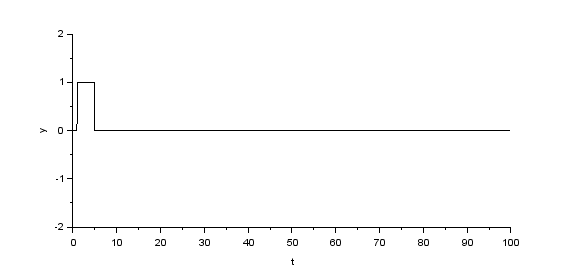
\includegraphics[width=0.8\textwidth]{amortiguador_entrada.PNG}
\caption{Señal ingresada al sistema que emla ser un lomo de burro}
\label{entrada}
\end{figure}

Para emular la perturbación producida por un lomo de burro, se ingresa al sistema una combinación de funciones escalón que dan como resultado la señal representada en la \mbox{figura \ref{entrada}}.\\

Las figuras \ref{KAC0}, \ref{KAC001}, \ref{KAC01}, \ref{KAC1}, \ref{KAC10} (a partir de la página \pageref{KAC0}) representan la altura del vehículo en relación al tiempo una vez pasado el lomo de burro, con constantes del cilindro que varían desde $0$ hasta $10$.\\

\begin{figure}[p]
\center
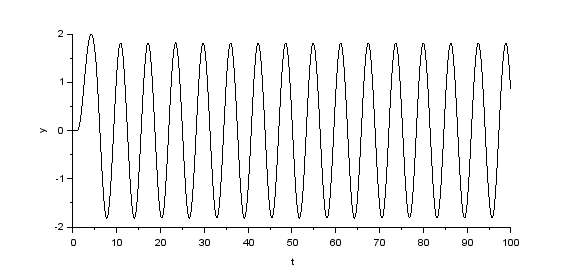
\includegraphics[width=0.8\textwidth]{amortiguador_0.PNG}
\caption{Función resultante con $K_{ac}=0$}
\label{KAC0}
\end{figure}

\begin{figure}[p]
\center
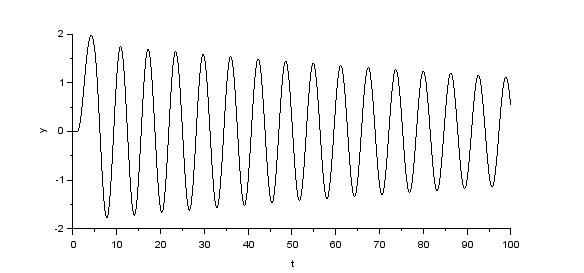
\includegraphics[width=0.8\textwidth]{amortiguador_001.PNG}
\caption{Función resultante con $K_{ac}=0.01$}
\label{KAC001}
\end{figure}

\begin{figure}[p]
\center
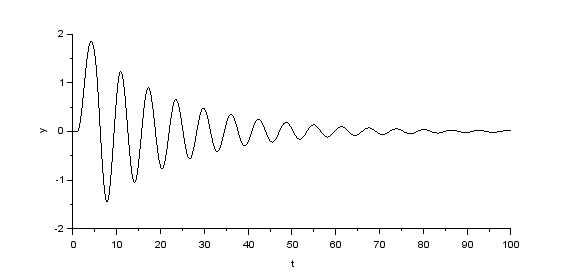
\includegraphics[width=0.8\textwidth]{amortiguador_01.PNG}
\caption{Función resultante con $K_{ac}=0.1$}
\label{KAC01}
\end{figure}

\begin{figure}[p]
\center
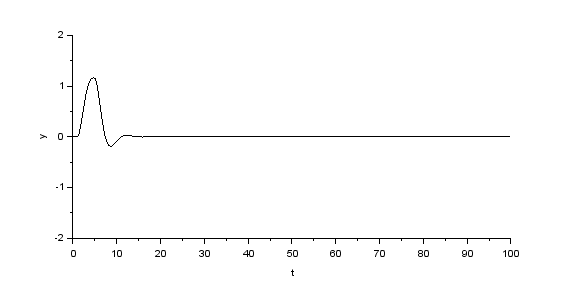
\includegraphics[width=0.8\textwidth]{amortiguador_1.PNG}
\caption{Función resultante con $K_{ac}=1$}
\label{KAC1}
\end{figure}

\begin{figure}[p]
\center
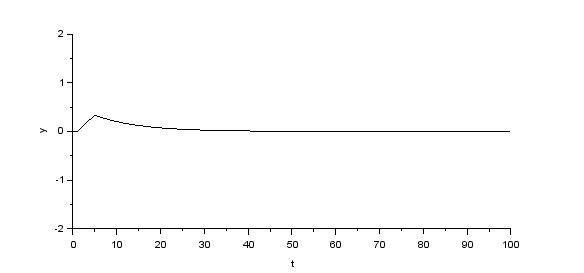
\includegraphics[width=0.8\textwidth]{amortiguador_10.PNG}
\caption{Función resultante con $K_{ac}=10$}
\label{KAC10}
\end{figure}

En las diferentes gráficas se pueden observar las diferencias entre los distintos valores de constante del cilindro hidráulico, siendo en el caso en que $K_{ac} = 0$ un sistema donde no se pierde energía por lo que la oscilación del vehículo nunca cesa. Caso contrario sucede cuando la constante del cilindro adopta valores mas significativos, haciendo que la energía sea dicipada mas rápidamente lo que produce en consecuencia una rápida amortiguación de la perturbación. Ninguno de los extremos es deseable, ya que si no se amortigua, la altura del vehículo oscilaría indefinidamente produciendo momentos en que la adhesión al suelo es nula, lo cual es una situación indeseable en todos casos y sobretodo en vehículos de competición. En el extremo en que el aceite dentro del amortiguador es infítamente viscoso, el amortiguador perdería toda capacidad de atenuar suavemente las perturbaciones, produciendo fuertes golpes que pueden causar daños físicos a la estructura del vehículo.\\

Si bien para elegir un óptimo se trata de elegir un valor intermedio, considero que no hay un valor óptimo absoluto para la constante del cilindro, sino que la constante dependerá de qué se quiere lograr. Si se desea una amortiguación suave se debe reducir la constante del cilindro, si se desea un rápido agarre al suelo se subirá el valor de dicha constante a costa de golpes más bruscos a la estructura del vehículo.


\subsection{Calle de adoquines}

Para simular una calle de adquines se sumaron 3 funciones senoidales de distintas amplitudes y frecuencias, valores que son sólo para hacer las pruebas y que carecen de un fundamento para su elección. 

\begin{figure}[h!]
\center
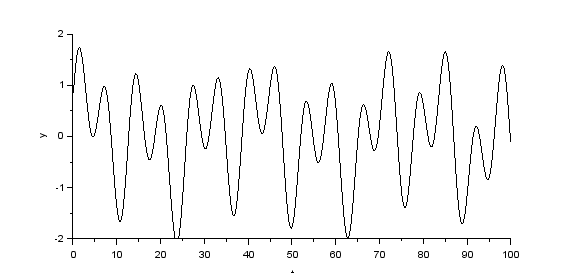
\includegraphics[width=0.8\textwidth]{adoquines_entrada.PNG}
\caption{Señal ingresada al sistema que emula una calle de adoquines}
\label{adoquines_entrada}
\end{figure}

En las imágenes \ref{adoquines_1} y \ref{adoquines_10} se puede observar la iferencia de comportamiento frente a una calle de adoquines, quedando prácticamente invariente la salida respecto  la entrada en el caso en que $K_{ac}=1$ (figura \ref{adoquines_1}) y atenuándose considerablente en el caso en que $K_{ac}=10$ (figura \ref{adoquines_10}).

\begin{figure}[p]
\center
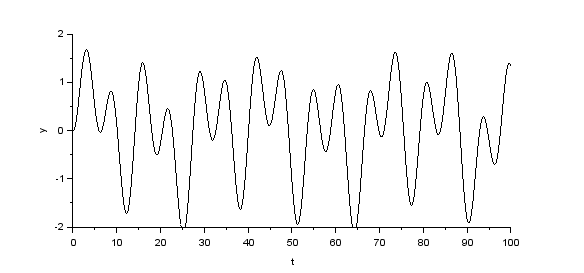
\includegraphics[width=0.8\textwidth]{adoquines_1.PNG}
\caption{Función resultante de calle de adoquines con $K_{ac}=1$}
\label{adoquines_1}
\end{figure}

\begin{figure}[p]
\center
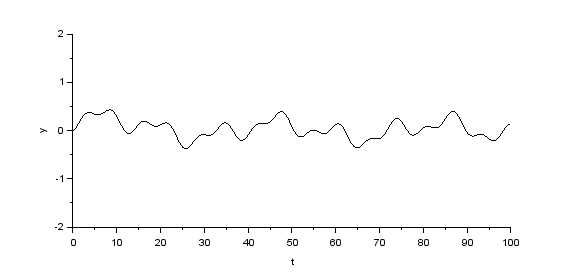
\includegraphics[width=0.8\textwidth]{adoquines_10.PNG}
\caption{Función resultante de calle de adoquines con $K_{ac}=10$}
\label{adoquines_10}
\end{figure}



\end{document} 